\documentclass[11pt,a4paper]{article}

\usepackage{Rapport_Type} %% cibler doc/modules/

\usepackage{fancyhdr}
\fancypagestyle{basdepage}{
\fancyhead{}
\fancyfoot{} % clear all footer fields
\fancyfoot[C]{Stage Lip6 : Amélioration de la réactivité des réseaux p2p pour les MMOGs (\thepage)}
\renewcommand{\headrulewidth}{0pt}
\renewcommand{\footrulewidth}{0pt}}
\pagestyle{basdepage}

\begin{document}
  \fairetitre{Amélioration de la réactivité des réseaux pair à pair pour les MMOGs}{Rapport Bibliographique}{Xavier Joudiou}{Sébastien Monnet \& Sergey Legtchenko}{29/04/10}

\newpage
\tableofcontents

\newpage
\section{Abstract}

	Depuis plusieurs années, une nouvelle classe d'application est apparue. Il s'agit des applications pair à pair, ces applications sont devenues populaires grâce à des applications de partage de fichier. De nombreuses autres utilisations de l'architecture pair à pair existent, comme pour la communication, la distribution de calculs scientifiques, les jeux vidéos multijoueur en ligne, etc. Nous allons nous intéresser aux jeux vidéos massivement multijoueur ( MMOG pour Massively Multiplayer Online Games) qui sont de plus en plus populaires et qui font ressortir des problèmes que l'architecture pair à pair doit pouvoir corriger. Le problème du passage à l'échelle sera l'un des plus importants à résoudre car des milliers de joueurs doivent pouvoir participer en même temps et avec un latence faible.\\ 
	L'architecture pair à pair est la plus adaptée pour résoudre le problème de passage à l'échelle dans les MMOGs, mais il sera plus difficile d'assurer une faible latence. Le but de ce stage est de proposer une technique efficace de prédiction du comportement des joueurs de MMOG afin de pouvoir anticiper leurs mouvements. Il est alors possible d’adapter le réseau en conséquence et ainsi diminuer la latence due au routage.\\ 
	A l'heure actuelle, les MMOGs utilisent une architecture client/serveur, ce qui pose des problèmes de passage à  l'échelle, car on aura un nombre de joueurs limités pouvant être sur chaque serveur. Ce qui fait que le jeu est découpé en plusieurs parties indépendantes, chacune étant gérée par un serveur, ce qui pose des problèmes d'unité de l'univers. Ce problème implique aussi un coût achat de serveur et en maintenance de ceux-ci très élevé.\\
	Pour remédier à cela, une solution consiste à remplacer le modèle client/serveur par un réseau logique pair à pair (overlay).Malheureusement, les protocoles pair à pair existants sont trop peu réactifs pour assurer la faible latence nécessaire à ce genre d’applications. En effet, pour une expérience de jeu satisfaisante, l’information entre deux pairs en interaction dans le MMOG doit être transmise avec une latence d’au plus quelques centaines de millisecondes. Ceci est problématique, même avec un routage efficace.\\
	Néanmoins, quelques travaux ont déjà été menés pour adresser ce problème. L’idée est d’adapter le voisinage de chaque pair afin que toute l’information dont il aura besoin dans un avenir proche se trouve à un seul hop de lui dans le réseau. Il est alors nécessaire de correctement évaluer les futurs besoins de chaque pair, et de faire évoluer son voisinage à temps.
		Le travail à réaliser est d'améliorer un overlay pair à pair pour MMOG qui a été implémenté dans le simulateur Peersim. Cet overlay anticipe les mouvements du joueur dans le MMOG et adapte le voisinage de son pair en conséquence. Cependant, les algorithmes d’anticipation sont naïfs et peu précis .
Il s’agit donc de concevoir des mécanismes efficaces d’anticipation de la trajectoire des joueurs afin de mieux adapter l’overlay à leurs déplacements et diminuer la latence.\\

\textbf{Mots Clés:} Pair à pair, Massively Multiplayer Online Games, Overlay, Anticipation des movements, Collaboration des nœuds ...


%\newpage
\section{Introduction}
	Le début de ce rapport va permettre d'observer les différents travaux déjà réalisés sur les applications pair à pair. Les jeux vidéos massivement multijoueur étant le principal type d'application qui va nous intéresser. Ces applications, regroupant un grand nombre de personnes, impliquent que différentes propriétés (jouabilité, fluidité, réactivité, etc) soient vérifiées. L'architecture pair à pair peut répondre efficacement à certaines des différentes propriétés nécessaires au bon fonctionnement des applications mais un problème peut se poser au niveau de la latence. Le but du stage a été d'améliorer le voisinage logique du réseau pair à pair pour que l'utilisateur puisse avoir dans son voisinage les données. Ces données lui seront nécessaires aux instants suivantes dans l'environnement, pour cela il faut anticiper au mieux les mouvements du joueur.\\

	Tout d'abord nous expliquerons pourquoi l'approche pair à pair est celle qui paraît la plus adaptée pour répondre aux différentes problématiques qu'induisent ces applications, nous en profiterons pour rappeler rapidement les caractéristiques des différentes architectures (cf \ref{whyp2p}, page \pageref{whyp2p}). Ensuite, les mécanismes permettant une meilleure mise en place de l'architecture pair à pair seront expliqués, nous rentrerons un peu plus dans les détails pour Solipsis (cf \ref{solipsis}, page \pageref{solipsis}). Solipsis est un travail qui propose un monde virtuel entièrement décentralisé et scalable. Un overlay qui est caractérisé par une forte malléabilité applicative, sert de support au monde virtuel. Après avoir parlé des différents mécanismes existants qui ne prennent pas en compte la mobilité, une étude des traces des avatars dans les environnements virtuels sera alors introduite (cf \ref{trace}, page \pageref{trace}). Cette étude des traces permettra de mieux expliquer les différentes solutions d'amélioration de la réactivité du réseau pair à pair. Ensuite, le travail Blue Banana qui a permis de mettre en place une première amélioration, au fonctionnement du monde virtuel proposé par Solipsis, sera expliqué (cf \ref{BlueBanana}, page \pageref{BlueBanana}). Blue Banana permet d'anticiper les mouvements des avatars, pour ainsi adapter au mieux le voisinage des nœuds. \\

	
	Ensuite, les deux principales améliorations, qui ont été mises en place durant ce stage, seront présentées. La première solution consiste à intégrer un cache dans les nœuds du réseau, son fonctionnement et ses performances seront expliqués. L'autre solution, implémentés durant le stage, est une amélioration du préchargement des données qui a été mis en place dans Blue Banana. Outre l'explication des résultats de chacune des solutions, les différentes implémentations explorées seront présentées. Enfin les autres pistes d'amélioration, qui ont été envisagées, seront expliquées.



%\newpage
\section{Présentation du Laboratoire d' Informatique de Paris 6}
	\subsection{Le laboratoire}
	Le LIP6 est un laboratoire de recherche sous tutelle de l'Université Pierre et Marie Curie, et du CNRS (UMR 7606). Avec 184 chercheurs permanents et 258 doctorants, il est l'un des principaux laboratoires de recherche en informatique en France. Une équipe administrative de 13 personnes et une équipe technique de 12 personnes en assure le fonctionnement. Le Directeur du laboratoire est Patrick Gallinari et le directeur adjoint est Pierre Sens. Le laboratoire vient de revenir à Jussieu après plusieurs années d'exil sur le site de Radio France Avenue de Président Kennedy dans le 16° arrondissement.

Le laboratoire couvre un large spectre d'activités regroupées au sein de cinq départements : Calcul Scientifique, DEcision, Systèmes Intelligents Recherche opérationnelle, Données et Apprentissage Artificiel, Réseaux et Systèmes Répartis, Systèmes Embarqués sur Puce. En complément de la recherche académique, le LIP6 a une longue tradition de coopération avec des partenaires industriels dans de très nombreux projets nationaux, européens ou internationaux. Deux centres R et D ont été créés : le CERME, Centre Européen de Recherche en Micro-Electronique sur les systèmes embarqués, et Euronetlab, sur l'internet et les réseaux de télécommunication. Le LIP6 est également impliqué dans les pôles de compétitivité de l'Ile-de-France : Cap Digital sur le contenu numérique et System@tic sur les systèmes embarqués.

Il a également des équipes communes avec l'INRIA sur les thématiques du calcul formel et des systèmes répartis. La coopération internationale est une constante pour les activités du laboratoire. Le LIP6 est membre de plusieurs réseaux d'excellence et développe également des relations suivies avec des universités au Brésil, aux États-Unis, au Japon, et dans de nombreux pays européens. Le laboratoire est largement ouvert aux projets de coopération et à l'accueil de visiteurs scientifiques. Le laboratoire est impliqué dans des enseignements liés à la recherche, qui sont dispensés au Master « Sciences et technologie » à l'Université Pierre et Marie Curie. L'EDITE de Paris (Ecole Doctorale d'Informatique, Télécommunication et Electronique de Paris) accueille nos doctorants.


	\subsection{L'équipe REGAL}
	L'équipe REGAL fait partie du département "Réseaux et Systèmes Répartis" qui est dirigé par Bertil Folliot. Le département "Réseaux et Systèmes Répartis" se concentre sur la conception de solutions pour construire et gérer les réseaux et systèmes du futur. Il est constitué de quatre équipes : MoVe (Modélisation et Vérification), REGAL (Répartition et Gestion des Applications à Large Echelle), NPA (Networks and Performances Analysis) et Phare. L'équipe REGAL est un équipe commune avec l'INRIA Rocquencourt, le responsable de cette équipe est Pierre Sens. L'objectif de l'équipe est la gestion de ressources dans le cadre très dynamique de grands réseaux. REGAL s'intéresse aux techniques de déploiement d'applications (code et données) adaptées aux environnements extrêmement distribués de grande taille (nombre de processeurs, distances), fortement dynamiques, hétérogènes, sans possibilité simple de gestion centralisée et/ou instantanée de la connaissance mutuelle. L'approche de REGAL repose sur des techniques de réplication et d'adaptation dynamique dans lesquelles un code applicatif et ses données sont dupliqués sur plusieurs sites ce qui permet de tolérer les fautes, d'augmenter la disponibilité et réduire les temps d'accès du service rendu par l'application. Nous étudions la façon dont les systèmes peuvent garantir une qualité de service en termes de fiabilité, disponibilité et cohérence.

	\vspace{1.5cm}
        \begin{figure}[!h]
        \centering
        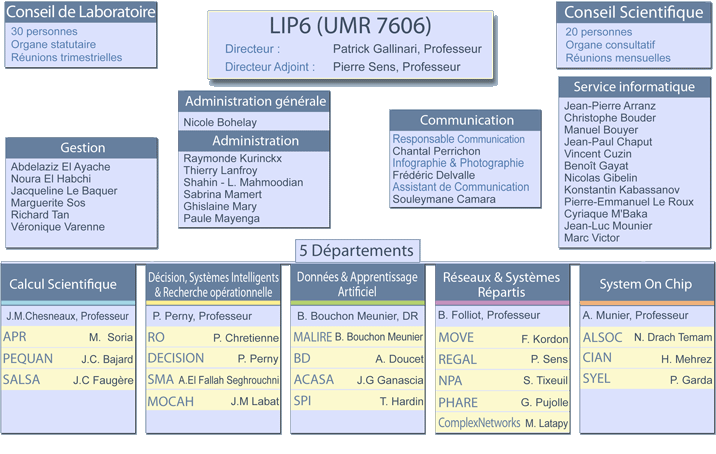
\includegraphics[width=15cm,height=8cm]{../Images/Lip6_Organisation.png}\\
        \caption{Schéma de l'organisation du LIP 6}
        \label{LIP 6}
        \end{figure}
	\vspace{1.5cm}

	\subsection{L'INRIA Paris - Rocquencourt}
	L’INRIA Paris - Rocquencourt est l'un des huit centres de recherche de l’Institut National de Recherche en Informatique et Automatique (INRIA), organisme de recherche spécialisé dans le domaine des Sciences et Technologies de l’Information et de la Communication. C'est un établissement public placé sous la double tutelle du ministère de la recherche et du ministère de l’économie, des finances et de l’industrie, l'INRIA accueille environ 3 800 personnes dont 2 800 scientifiques. 
	Combiner l’excellence scientifique et le transfert technologique est le fondement de la stratégie de l’institut, dans laquelle s’inscrit en particulier le centre de recherche INRIA Paris - Rocquencourt. Ainsi, ses objectifs prioritaires de recherche - réseaux et systèmes de communication - logiciels fiables et sécurité - modélisation du vivant et de l'environnement – sont conduits avec le souci de concilier recherche en amont du meilleur niveau international, applications et valorisation par le biais d’interactions constantes avec le monde socio-économique.

Ils mènent ses activités scientifiques en développant des partenariats étroits avec les équipes internationales de pointe, le monde de l’industrie et des services, en particulier dans le cadre des pôles de compétitivité, et de nombreux établissements d’enseignement supérieur et de recherche d’Île-de-France.
	


\newpage
\section{Pourquoi passer à des solutions pair à pair?}
	\label{whyp2p}
	Nous allons voir pourquoi est-il nécessaire de passer d'une architecture Client/Serveur à une architecture pair à pair, nous verrons les différences des deux solutions.
	\subsection{Les solutions existantes}
	Dans la plupart des Massively Multiplayer Online Games, l'architecture est de type client/serveur (voir page ~\pageref{P2P/ClServ}). Dans cette architecture, il a forte distinction entre le client, qui envoie des requêtes au serveur et attend les réponses, et le serveur qui est à l'écoute de requêtes des clients. Cela va simplifier la sécurité et le fonctionnent global des jeux. Par exemple, pour effectuer des updates sur l'état global du jeu, il suffit de le faire sur un seule machine et il n'y aura pas de problème d'incohérence entre les données. De même pour la sécurité, toutes les données étant regroupées sur une seule machine, le contrôle sera beaucoup plus simple que dans des systèmes distribués où le nombre de point d'entrée sera beaucoup plus important. \\
	Le problème est que cette architecture ne passent pas à l'échelle, le serveur devient un goulot d'étranglement et si un trop grand nombre de joueurs se connecte, le serveur ne tiendra pas. Le problème est résolu "temporairement?" en ayant des serveurs de très grandes capacités ou en mettant en place des clusters de serveur \textbf{(voir bibli)}. Mais ces solutions induisent un gros investissement dès le début de la mise en service du jeu et elles sont très chères en coût de maintenance. Un autre problème est le disponibilité du système en cas de panne du serveur, si le serveur tombe en panne alors plus personne n'aura accès à l'application que ce dernier faisait fonctionner. \\
	Au vue du nombre croissant de participant à ce genre de jeux vidéos massivement multi joueur, le passage à l'échelle devient un sujet très important et c'est pour cela que les recherches sur des architectures distribuées sont de plus en plus importantes textbf{(voir si statistiques)}. \\
\newline


	\subsection{Les avantages et les inconvénients du pair à pair}
	Comme il est dit avant, l'augmentation croissante des recherches sur le sujet atteste du fait que des problématiques ressortent des solutions existantes. Le problème du passage à l'échelle est sûrement le plus important et est l'une des raisons de ces recherches. Les architectures pair à pair ne font plus ressortir d'entité serveur et client, chaque nœud sera client et serveur en fonction du moment (voir page ~\pageref{P2P/ClServ}). Les systèmes pair à pair peuvent avoir une multitude d'utilisation, que ce soit dans le partage de fichier, la communication, les jeux vidéos , le calcul scientifique, le militaire, etc. \\
	L'architecture pair à pair est faite telle qu'il n'y a pas de goulot d'étranglement, nous passons d'un système où tout passait par un point unique à un système qui comporte un grand nombre d'entité qui peuvent toutes avoir le même rôle. L'utilisation de cette architecture peut entrainer un grand nombre de communications, elle nécessite des synchronisations des entités, des gestions des ressources partagées et d'autres problèmes ( \textbf{A REVOIR}), il faut donc trouver des solutions à tous ces problèmes éventuels. Elle est donc plus adapté à des applications massivement multi joueur mais il faut pouvoir garantir les mêmes propriétés que les systèmes client/serveur. A REVOIR\\
	Les systèmes pair à pair sont par exemple plus difficile à surveiller, les phénomènes de tricherie sont plus difficiles à surveiller, de même pour tout ce qui est sécurité. Nous avons pu voir qu'il existe trois type de tricherie: par Confidentialité, c'est à dire d'obtenir des informations non autorisées sur d'autres utilisateurs; par Intégrité, si il y des modification du monde, des lois physiques ou les lois du jeu non autorisées; par Availability, c'est le fait de provoquer des ralentissements ou des arrêts de parie du jeu ( référence vers Challenges in P2P gaming). Il faut que le système soit aussi fiable sur le long terme et qu'il soit tolérant aux connexions et déconnexions.

\\ \newline
	
	AJOUTER. Les jeux vidéos ont des avantages qui font qu'il sera plus aisé de réaliser une distribution~\cite{1267692}:
	\begin{itemize}
		\renewcommand{\labelitemi}{$\bullet$}
		\item Les jeux vidéos tolèrent une consistence faible pour les différents états de l'application.
		\item Il est assez aisé de prédire les écritures et les lectures grâce à l'ensemble des règles définies dans le jeu. 
	\end{itemize}
	\vspace{1.5cm}
	\begin{figure}[!h]
	\centering
	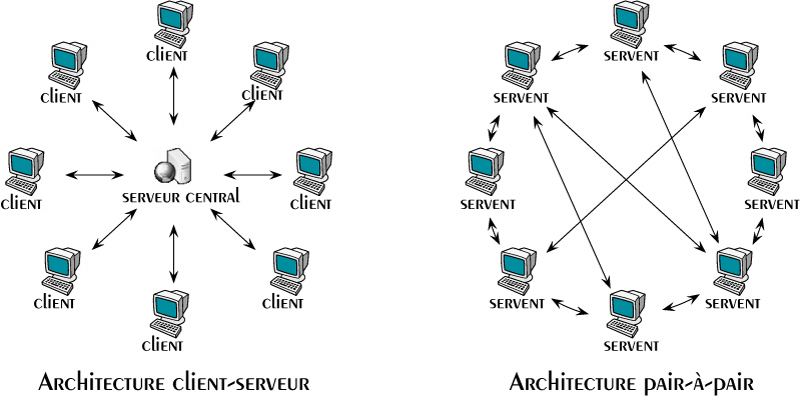
\includegraphics[width=15cm,height=8cm]{../Images/p2p-85145.png}\\
	\caption{Schéma des architectures pair à pair et client/serveur}
	\label{P2P/ClServ}
	\end{figure}


\newpage
\newpage
\section{Traces des utilisateurs dans les MMOGs}
	\label{trace}
 	Après avoir exposées des solutions qui ne prennent pas en compte la mobilité des joueurs, nous allons étudier celle-ci pour introduire la solution proposé par le travail Blue Banana. Pour étudier la mobilité dans les MMOGs, différentes techniques de collecte de traces ont été mises en place, nous présenterons celles-ci et expliquerons pourquoi ce travail de collecte est important pour améliorer les performances des solutions pair à pair pour les MMOGs.
	\subsection{Les différentes techniques de récupération de trace}
		\subsubsection{Les objectifs et les techniques de collecte de trace}
		\par Dans la littérature, il y a plusieurs études des traces d'utilisateurs de différents environnements virtuels~\cite{1326262,0295-5075-88-4-48007}. La plupart vont récupérer les traces des avatars sur des jeux vidéos tel que World Of Warcraft~\cite{wow} et Second Life~\cite{sl}. Ces études expliquent qu'il peut y avoir des différences entre des MMOGs. Par exemple dans Second Life l'environnement est beaucoup plus interactif (possibilités plus étendues de modification de l'environnement) que dans World Of Warcraft, ce qui peut affecter des différences de résultats des solutions en fonction du jeu~\cite{DBLP:journals/corr/abs-0807-2328,1613041}. \\
\par Ces travaux permettent de bien comprendre les différents comportements des joueurs, ils permettent ainsi de détecter les différents comportements en fonction des zones plus ou moins peuplées. Grâce à ces travaux, il est possible de faire ressortir des modèles montrant le comportement des avatars dans le monde virtuel. Ces modèles permettent de mettre en place une distribution spatiale des avatars, qui sera plus cohérente que dans les recherches où les distributions étaient uniformes~\cite{Knutsson04peer-to-peersupport}. Différentes mesures vont apparaître comme: le nombre de joueurs, le nombre d'arrivées et de départs, le temps moyen d'une session, la distribution des joueurs, etc. L'étude des traces des joueurs permet aussi de détecter les tricheurs qui utilisent souvent des bots~\cite{0295-5075-88-4-48007}. \\
		%\subsubsection{Les techniques de collecte des traces}
	\par Certaines techniques utilisent un bot qui est introduit dans le jeu et qui va récupérer des informations sur les autres joueurs. Le bot va rapatrier des informations à intervalles réguliers, il sera alors possible d'analyser les déplacements et vérifier les modèles. Une librairie open source \textit{libsecondlife} a été développée pour collecter les traces des joueurs de Second Life, à l'aide d'un bot~\cite{DBLP:journals/corr/abs-0807-2328}. Pour vérifier que les données récupérées sont cohérentes, une technique de positionnement de sept bots dans une région a été mise en place. Quatre bots statiques sont placés à chaque coin de la région, un autre statique va se placer au centre et deux autres vont bouger suivant un schéma défini. Il est alors possible d'enregistrer les positions des avatars se trouvant dans la région et les enregistrements des informations seront réalisés sept fois (par chaque bot). Une comparaison des données des sept bots est alors effectuée pour voir si des déviations existent entre les valeurs et si elles sont importantes.\\  
 		\subsubsection{Limitations de la collecte des traces}
	Des limitations existent pour la collecte des traces. Une des premières est que les mondes virtuels sont très souvent découpés en région ou en île, or les bots que nous introduisons ne peuvent pas traverser les régions et ils ne peuvent pas, par exemple, suivre des avatars. Dans~\cite{DBLP:journals/corr/abs-0807-2328}, la possibilité de différencier un avatar qui va dans une autre région et un qui quitte le jeu n'est pas possible. Il n'est pas possible de savoir ce que va faire l'avatar en dehors de la zone. Il y aussi un problème avec la détection des avatars qui se trouvent sur des objets et il n'y pas de prise en compte de la coordonnée \textit{z}. Une autre limitation de la collecte des traces est qu'elle se fait en très grande majorité de façon manuelle, il est donc très long et fastidieux de récupérer un nombre de traces suffisant pour effectuer des bonnes analyses. La collecte de trace peut aussi avoir des problèmes de passage à l'échelle car les systèmes de collecte existants travaillent à une petite échelle. Par exemple dans Second Life, le monde étant découpé en îles indépendantes, l'addition des traces collectées sur chaque île pour en faire une étude globale, n'est pas cohérente.

	\subsection{Observations des traces}
	 Beaucoup d'observations sur les déplacements des avatars dans les mondes virtuels ont pu être réalisé grâce à la collecte de toutes ces traces. La collecte des traces a aussi permis de faire valider ou invalider des modèles qui avaient été mis en place sans étude des traces~\cite{DBLP:journals/corr/abs-0807-2328}. 
		\subsubsection{Hotspots}
	Une des observations qui est ressortie de ces études est l'existence de différentes zones dans le monde. Une autre observation est que les mouvements des avatars sont très différents en fonction de la zone où ils se trouvent. Deux types de zones peuvent se dégager: des zones très peuplées avec des avatars ayant des mouvements très aléatoires et lents (Hotspots), et des zones qui sont entre les zones peuplées, où les avatars se déplacent rapidement et suivent souvent une trajectoire rectiligne (Waypoints). Des phénomènes de déplacement en groupe ont aussi pu être repérés~\cite{15141312}. \\
		\subsubsection{Waypoints}
	Comme nous pouvons le voir dans le schéma~\ref{sch_trace}, il y a des "routes" entre les différents points de regroupement. Ces routes vont nous permettre de mieux anticiper les déplacements des avatars entre les \textit{Hotspots}.
        \vspace{1mm}
        \begin{figure}[!h]
        \centering
        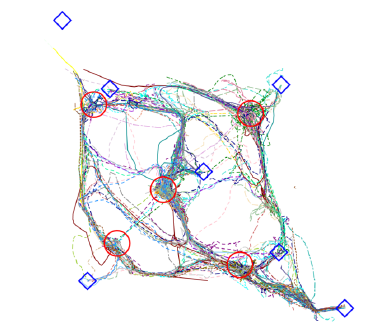
\includegraphics[scale=0.75]{./Ressources/Images/trace.png}\\
        \caption{Battle 980 movement paths}
        \label{sch_trace}
        \end{figure}	
        \vspace{1mm}
\newline
	L'étude des traces a aussi permis de détecter les habitudes des joueurs, comme le fait qu'ils jouent à certaines heures plutôt que d'autres et avec des durées de connexion différentes en fonction de l'heure de la journée.


\newpage
\section{Mécanismes d'amélioration existants}
	\subsection{Area Of Interest}
	Dans plusieurs articles, la notion de \textit{Area Of Interest}~\cite{1403002,1267692,1015507} va apparaître ce qui montre l'utilité de ce mécanisme. Nous pouvons déjà retrouver ce principe sous le nom de \textit{Local Awareness} dans Sollipsis, l'idée principale de ce mécanisme est qu'une entité n'a pas besoin de connaître l'ensemble du monde virtuel à chaque instant. Alors nous allons mettre en place une zone dans laquelle l'entité sera tenue informée des différentes modifications qui seront faites sur les objets et les autres entités qui se trouvent dans la zone (voir schéma~\ref{AOI}). Si une entité modifie sa représentation virtuelle, seulement les entités qui sont dans sa zone seront directement informées.\\

	%\subsubsection{Mercury}
	\par Dans Mercury~\cite{1015507}, le concept d'Area Of Interest va pouvoir être utile avec le mécanisme de publish-subscribe qui est mis en place. Ce mécanisme de publish-subscribe permet l'abonnement et le désabonnement aux mises à jour d'un objet, et il permet donc d'envoyer un objet vers les nœuds qui sont abonnés.\\
	%\subsubsection{Colyseus}
	\par Colyseus~\cite{1267692} est un travail postérieur à Mercury, les principes sont les mêmes avec l'utilisation de \textit{range-queriable} DHT ou de DHTs pour stocker les informations. Les \textit{range-queriable} DHTs vont s'organiser en un overlay circulaire où chaque nœud adjacent est responsable d'une suite continue de clés. Grâce à cela, il sera possible de prendre les coordonnées "x" comme clé et ainsi les performances seront bien meilleures qu'avec des DHTs normales (aléatoire). Les différents résultats réalisés montrent bien que les \textit{range-queriable} DHTs utilisent moins de bande passante que les DHTs normales. \\
	%\subsubsection{Donnybrook}
	\par Dans Donnybrook~\cite{1403002}, le concept d'Area Of Interest fait référence au travail réalisé dans Colyseus. Comme chaque joueur envoie ses mises à jour à chaque joueur qui se trouve dans sa zone, il faut une limitation du nombre de joueurs dans une même zone. Donnybrook introduit la notion de \textit{player's interest set}, un joueur va pouvoir se concentrer sur un nombre fixe de joueur (cinq dans l'article), à la différence du nombre d'objet dans l'AOI qui peut varier. Un mécanisme d'abonnement sera mis en place pour s'échanger les informations entre les joueurs. Un mécanisme d'\textit{intérêt estimé} est mis en place pour définir les joueurs qui feront partis de son \textit{interest set}. Plusieurs critères sont pris en compte pour choisir les joueurs qui seront sélectionnés. Trois principales propriétés sont prises en compte: la proximité spatiale entre les joueurs, les objectifs des joueurs et les interactions récentes que les joueurs peuvent avoir eu entre les deux joueurs.\\
	\vspace{5mm}
        \begin{figure}[!h]
        \centering
        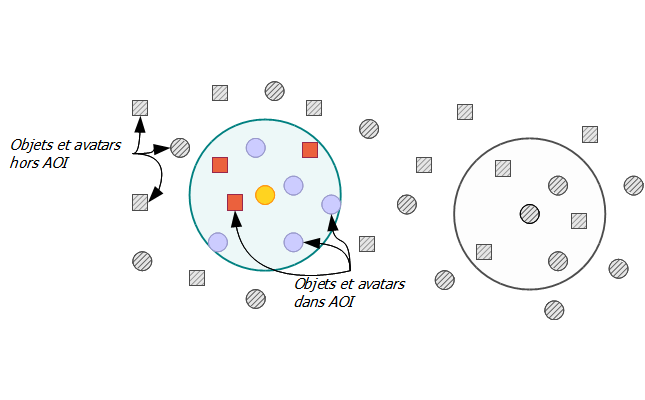
\includegraphics[scale=0.65]{../Images/AOI.png}\\
        \caption{Principe de l'\textit{Area Of Interest}}
        \label{AOI}
        \end{figure}
	\vspace{5mm}
	\subsection{Découpage de la carte}
	Pour plusieurs raisons, dont la tenue en charge, le monde a été découpé en plusieurs zones. Différentes techniques pour le découpage ont été étudiées, l'une des plus courantes est d'utiliser le découpage grâce au découpage de Voronoi~\cite{1016552}, c'est de cette technique que la triangulation de Delaunay s'inspire. Les découpages suivant ces principes sont répandus car un découpage aléatoire ne prendrait pas en compte la densité des objets dans le monde qui peut être très variable entre les régions. Le principe est de découper la monde en zone en fonction de la distance entre les différents objets qui se trouvent dans l'environnement. Dans une région, on aura un objet qui sera entouré de ses voisins. La frontière entre la région de deux voisins se trouve au milieu d'une droite séparant les deux voisins. Comme il est possible de voir sur le schéma~\ref{Voronoi}, les zones ont des formes et des tailles qui sont différentes. Nous avons ainsi des zones qui comprennent un seul nœud. La différence entre la triangulation de Delaunay et le découpage de Voronoi est que pour la première, les arrêtes seront les droite entre les sommets si ils sont voisins et dans le deuxième cas, les arrêtes seront formés grâce aux médiatrices des arrêtes de la triangulation de Delaunay.\\ 
	\vspace{5mm}
        \begin{figure}[!h]
        \centering
        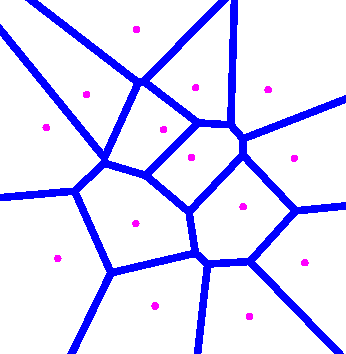
\includegraphics[scale=0.45]{../Images/voronoi.png}\\
        \caption{Principe du découpage de Voronoi}
        \label{Voronoi}
        \end{figure}
        \vspace{5mm}

	\subsection{Overlays}
	Plusieurs travaux sur la modification de l'overlay ont été fait~\cite{999375,10.1109/SRDS.2006.33,citeulike:6040284}, le but principal de ces travaux est de mettre en place un overlay qui puisse facilement s'adapter aux besoins des nœuds.
		\subsubsection{Semantic overlay}
			Le but principal de cet overlay sémantique~\cite{999375} est de créer des liens entre des nœuds qui s'intéressent aux mêmes documents, car la recherche de fichiers est devenu très importante au moment de l'arrivée des logiciels de partage de fichiers tel que Napster, Gnutella, KaZaA, etc. L'approche consiste à constituer des groupes sémantiques avec les documents et de construire un overlay au dessus du réseau pour chaque groupe. Le problème est donc d'identifier et de constituer des groupes efficacement. Trois stratégies ont été mises en place:
		\begin{itemize}
		\renewcommand{\labelitemi}{$\bullet$}
                	\item \textit{LRU:} Stratégie basé sur les éléments les plus récemment utilisés
                	\item \textit{History:} On maintient les liens sémantiques vers la même classe de préférence, cette technique oblige le maintien d'un nœud \textit{counter}.C'est une technique lourde en nombre de messages et en stockage, de plus il peut y avoir des problèmes avec les \textit{counters}.
	                \item \textit{Popularity:} Création de liens entre les nœuds du même type, introduction de deux paramètres: Numrep (nombre de réponse positive pour obtenir le document) et Lastreply (date de la dernière réponse )
        	\end{itemize}
	        Les résultats montrent que Popularity est l'algorithme le plus adapté, cette stratégie a un bon compromis entre efficacité et complexité de mise en place.

		\subsubsection{Application-Malleable Overlay}
			Il y a deux types d'overlay (structuré et non structuré), mais ces deux types ont un désavantage commun, ils ne sont pas flexibles. MOve~\cite{10.1109/SRDS.2006.33} souhaite mettre en place un overlay malléable, c'est à dire que les communications de l'application distribué vont influencer la structure de l'overlay. Les deux buts principaux sont d'optimiser les performances de l'overlay et de garder les propriétés de tolérance aux fautes et de passage à l'échelle. Les auteurs mettent en place deux types de liens:
		\begin{itemize}
	        \renewcommand{\labelitemi}{$\bullet$}
	                \item \textit{Lien non-applicatif:} Ils maintiennent l'overlay global proche d'un graphe aléatoire avec un faible degré de clustering (regroupement).
        	        \item \textit{Lien applicatif:} Ils  permettent de créer un graphe fortement connecté, pour regrouper les nœuds. Chaque nœud d'un groupe crée aléatoirement des liens applicatifs vers des membres du groupe. Cela va permettre une rapide propagation des états lors des updates et des messages applicatifs multicast.
        	\end{itemize}
        Cette solution offre différentes possibilités d'ajout de nœud, de détection de défaillance, de remplacement de lien, etc. \textit{group}-based applications influencent l'overlay sous-jacent en remplaçant les liens inter nodes par des liens entres les applications. L'algorithme maintient une bonne connectivité.
		\subsubsection{Voronoi-based Overlay Network}
		 	VON veut exploiter la localité des intérêts des utilisateurs pour maintenir la topologie pair à pair avec un faible \textit{overhead}. VON utilise un principe d'AOI dynamique, il utilise le découpage de Voronoi et chaque nœud est représenté par un site dans le diagramme. VON introduit trois procédures principales :
		\begin{itemize}
	        \renewcommand{\labelitemi}{$\bullet$}
                	\item \textit{Join Procedure:} Le textit{joining node} contacte le server pour avoir un ID unique, puis envoie une requête avec ses coordonnées à tous les nœuds existants. Création de la liste des voisins, mis à jour chez les voisins, etc.
                	\item \textit{Move Procedure:} Lorsque un nœud bouge ses coordonnées sont mises à jour chez ses voisins (gestion si nœud est à la limite de la région, si il y a des nouveaux voisins, etc).
                	\item \textit{Leave Procedure:} Le nœud se déconnecte (qu'importe sa raison et la manière) et ses voisins vont se mettre à jour.
        	\end{itemize}
        	VON permet de gérer un grand nombre d'utilisateurs et de garder un topologie consistante. Il y a beaucoup de messages introduits par l'AOI et si la vitesse des utilisateurs est trop importante, on a des problèmes pour notifier les nouveaux voisins.

		

	


\newpage
\section{Un système P2P pour MMOG: Solipsis}
	\label{solipsis}
	Solipsis est le ``socle'' du travail Blue Banana~\cite{keller-solipsis}, il est donc nécessaire de présenter les points importants pour la compréhension du travail Blue Banana. Solipsis introduit des propriétés qu'il va être important de comprendre et qui serviront lors de l'analyse des résultats des solutions implémentées durant le stage.
	\subsection{Introduction sur Solipsis} 
	\par Pour commencer, le fonctionnement global et les fonctionnalités importantes de Solipsis vont être présentés. Solipsis est fait pour accepter un nombre illimité d'utilisateurs et pour maintenir une cohérence suffisante pour un bon fonctionnement du système. Il peut être accessible par n'importe quel ordinateur, il peut fonctionner sur des ordinateurs peu puissants et avec des connections internet faibles (56Kbs) ou sans fil. Une fois les nœuds connectés, ils peuvent échanger des données telles que de la vidéo, du son, le mouvement d'avatar ou toutes choses affectant la représentation du monde virtuel. \\
	\subsection{Propriétés de Solipsis}
	Le monde de Solipsis est un tore à deux dimensions, chaque entité détermine sa position dans le monde et elle est responsable de cette dernière. Chaque utilisateur collecte les informations lui permettant de reconstituer son environnement virtuel local. Les connections entre les nœuds sont bidirectionnelles. 
		\subsubsection{Propriétés}
	Solipsis doit permettre aux utilisateurs de se déplacer à travers le monde, il faut pour cela que les deux propriétés locales suivantes soient respectées.
	\begin{itemize}
	\renewcommand{\labelitemi}{$\bullet$}
		\item \textit{Local Awareness:}\\
		Une entité doit être connectée avec tous ses plus proches voisins. Il est important de noter qu'une entité a la possibilité de connaître des entités en dehors de son environnement virtuel local. En revanche, cette propriété impose qu'une entité située à l'intérieur fasse partie des voisins de l'entité.	
		\item \textit{Global Connectivity:}\\
		Toute entité virtuelle doit se trouver à l'intérieur de l'enveloppe convexe contenant l'ensemble de ses voisins logiques. L'enveloppe convexe des entités est le plus petit polygone convexe formé par cet ensemble. Un mécanisme pour éviter qu'une partie du graphe soit isolée a aussi été mis en place.\\

		%Une entité doit connaître toutes les entités se trouvant dans son "champs de vision". Elle doit pouvoir détecter l'arrivée ou le départ d'une entité de son "champs de vision". Cette propriété est basée sur la Géométrie Informatique, elle assure qu'une entité ne "tourne pas le dos" à une partie du monde. L'enveloppe convexe des entités est le plus petit polygone convexe formé par cet ensemble. Un mécanisme pour éviter qu'une partie du graphe soit isolée a aussi été mis en place.\\
	\end{itemize}
        \vspace{1cm}
	\begin{figure}[!h]
	\centering
        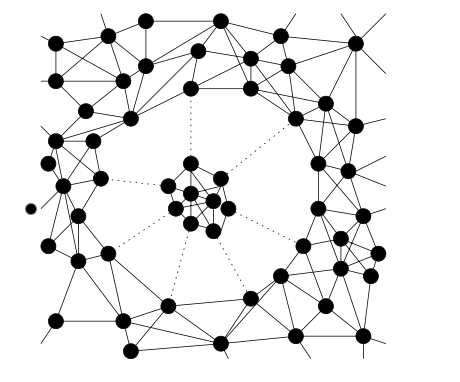
\includegraphics[scale=0.9]{./Ressources/Images/composant_isole1.png}\\
        \caption{Un composant connexe isolé et les connexions qui évitent la création d'une île}
        \label{Envelop_Convex}
        \end{figure}

		\subsubsection{Maintien des propriétés}
Solipsis a aussi des mécanismes de collaboration pour maintenir les propriétés précédentes, nous allons voir ces deux propriétés:
	\begin{itemize}
	\renewcommand{\labelitemi}{$\bullet$}
		\item \textit{Spontaneous Collaboration for Local Awareness:}\\
		 Pour vérifier la propriété \textit{Local Awareness}, il faut qu'une entité puisse connaître tous ses voisins à chaque instant. Pour faciliter cette connaissance du voisinage, et comme il y a un grand nombre de mouvements dans le monde virtuel, un système de collaboration entre les nœuds a été mis en place. Une entité pourra alors demander régulièrement à ses voisins s'ils détectent une nouvelle entité mais cela implique un grand nombre de messages inutiles et une perte temporelle de consistence. Pour éviter ces problèmes, une entité \textit{a} va prévenir une entité \textit{b} si une entité \textit{c} est en train de se diriger vers la zone de l'entité \textit{b}.
		\item \textit{Recursive Query-Response for Global Connectivity:}\\
		Il faut prévoir un mécanisme pour le maintien d'une entité dans l'enveloppe convexe. Quand une entité \textit{e} détecte deux entités consécutives, elle se lance immédiatement à la recherche d'une ou plusieurs entités dans la même zone en envoyant des messages dans la zone. \\ 
	\end{itemize}
        \vspace{1cm}
        \begin{figure}[!h]
	\centering
        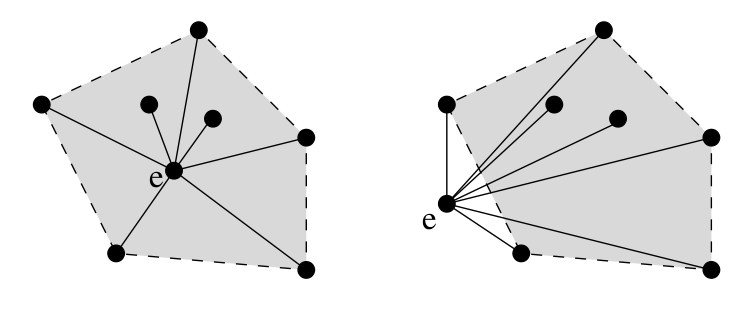
\includegraphics[scale=0.9]{./Ressources/Images/envelop_convex1.png}\\
        \caption{Deux différentes enveloppes convexes des voisins de \textit{e}. A gauche, \textit{e} respecte la règle de \textit{Global Connectivity} et à droite non.}
        \label{Envelop_Convex}
        \end{figure}


\newpage
\section{Prise en compte de la mobilité: Blue Banana}
	\label{BlueBanana}
	Il nous a été possible de voir, dans les chapitres précédents, des mécanismes qui permettent de faire évoluer le système en réaction à des événements. Solipsis ne pourrait difficilement fonctionner dans un monde avec des traces réalistes. En prenant en compte les études des traces des joueurs, Blue Banana a permis de mettre en place un mécanisme d'anticipation des mouvements des avatars pour mieux s'adapter.
	\par Blue Banana présente une solution aux différents problèmes que peut rencontrer une architecture pair à pair dans les MMOGs. La mobilité des avatars implique de nombreux échanges de données à travers le réseau pair à pair. Comme les overlays de l'état de l'art n'anticipent pas cette mobilité, les données nécessaires ne seront pas chargées à temps, ce qui conduit à des défaillances transitoires au niveau applicatif. Blue Banana a été réalisée pour résoudre ce problème, il modélise et prédit les mouvements des avatars ce qui permet à l'overlay de s'adapter par anticipation aux besoins du jeux.
	\subsection{Solutions introduites}
	Blue Banana est implémenté au dessus de Solipsis qu'il a été possible d'étudier dans le chapitre~\ref{solipsis}. Plusieurs observations ont été faites et différentes optimisations en sont ressorties. Il nous a été possible d'observer plusieurs types de zone (dense ou non, cf.~\ref{trace}) et que les mécanismes d'adaptation sont trop tardifs pour être mis en place dans la réalité (le chargement des données sera trop lent).
	\subsubsection{Les états de l'avatar}
	\label{Automate}
	Une des premières innovations qui a été introduite est la distinction de plusieurs états d'un avatar. Comme il a été possible de voir dans le chapitre sur la collecte de traces, un avatar se comporte différemment en fonction des zones du monde. Trois états ont donc été introduits:
	\begin{itemize}
	\renewcommand{\labelitemi}{$\bullet$}
		\item \textbf{H}(alted): l'avatar est immobile.
		\item \textbf{T}(ravelling): l'avatar se déplace rapidement sur la carte et il a une trajectoire droite.  
		\item \textbf{E}(xploring): l'avatar est en train d'explorer une zone, sa trajectoire est confuse et sa vitesse est lente.
	\end{itemize} 
	Le changement d'état de l'avatar se fait en fonction de la vitesse de celui-ci, si la vitesse devient supérieure à une borne définie et que l'avatar est dans l'état E alors l'avatar passe en état T. Ce modèle pourrait être affiné par la suite en prenant en compte l'accélération ou l'historique des mouvements. Sur la figure~\ref{automateMob}, nous pouvons mieux distinguer les différents changements d'état. Chaque nœud va agir en fonction de cette automate, il sera initialisé à l'état \textbf{H}(alted). \\
	

	\begin{figure}[!h]
        \centering
        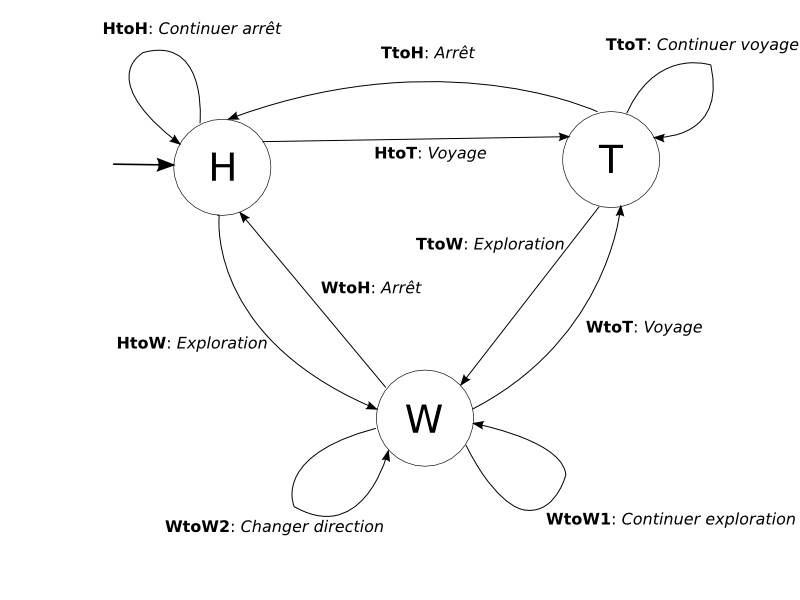
\includegraphics[scale=0.4]{./Ressources/Images/automate.png}
        \caption{\textit{\small Automate décrivant les mouvements d'un avatar. \textbf{En gras}: le nom de la transition, en \textit{italique} sa sémantique}}
        \label{automateMob}
        \end{figure}




	\subsubsection{Anticipation des mouvements}
	Un autre mécanisme a été mis en place, il s'agit d'anticiper les mouvements d'un avatar, pour cela deux suppositions sont faites: seulement une prédiction courte est cohérente, et plus l'avatar se déplace rapidement, plus il y a de chance qu'il continue dans la même direction~\cite{191}. Comme nous pouvons voir sur la figure~\ref{Propa_Algo}, en fonction du vecteur de mouvement de l'avatar, le nœud B, s'il est dans l'état \textbf{T}, va chercher des nœuds qui se trouvent sur la trajectoire probable de l'avatar, tant que son ensemble de voisins n'est pas plein. Le nœud B va envoyer un message aux voisins qui sont le plus près de lui par rapport au vecteur de mouvement. Un mécanisme pour évaluer si le nœud n'est pas trop près, et donc rapatrier des données ne servirait pas car le temps des communications serait supérieur au temps du déplacement de l'avatar. Un des risques est de rapatrier des nœuds qui seront inutiles si l'avatar va changer de direction ou d'état. L'amélioration de ce point fait parti des futures pistes pour améliorer l'algorithme d'anticipation des mouvements.\\
	\vspace{5mm}
        \begin{figure}[!h]
        \centering
        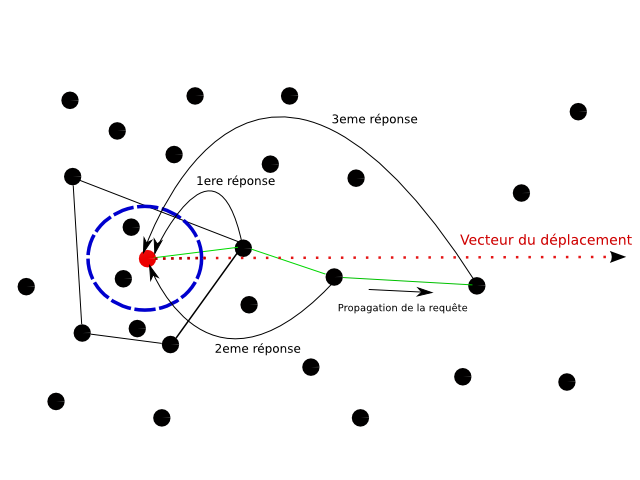
\includegraphics[scale=0.5]{./Ressources/Images/propagation_algo.png}\\
        \caption{Algorithme de propagation}
        \label{Propa_Algo}
        \end{figure}
        \vspace{5mm}
	\subsection{Expérimentations et Résultats}
		Le travail a été testé sur le simulateur à évènements discrets PeerSim ~\cite{peersim}, les expérimentations ont eu pour objectif de comparer Solipsis avec et sans Blue Banana.
		\subsubsection{Le simulateur PeerSim et la description des expérimentations}
		\par PeerSim est un simulateur de réseau pair à pair, qui a deux modes de fonctionnement: par cycles ou par évènements. C'est une API riche et modulaire qui est codée en Java, c'est une composante du projet BISON de l'université de Bologne (Italie). Ce simulateur permet de simuler un large nombre de machines et de tester différentes configurations du réseau. Le simulateur va faire des simplifications sur les couches réseau et les contraintes physiques (latence, pannes, ...). Chaque nœud est considéré comme un module qui va échanger des messages avec les autres nœuds du système. La plupart des plateformes de simulation est basée sur le modèle à évènements discrets. Il est possible de distinguer deux entités: les nœuds et les messages. Le temps va seulement évoluer à chaque nouvel évènement sur un nœud.
		%\subsubsection{Description des expérimentations}
		\par Au départ de la simulation, une carte initiale des traces est introduite dans le simulateur, la carte provient d'une étude de La et Michiardi~\cite{LM-wosn08} dans Second Life. Ensuite, le simulateur va initialiser l'overlay de Solipsis et vérifier que les deux règles de Solipsis sont bien respectées sur chaque nœud, nous insérerons ensuite le reste des traces. Il faut aussi régler les différents paramètres du simulateur (nombre d'avatar, surface du monde, densité, accélération des avatars, vitesse de connection, etc). Plusieurs métriques sont mises en place pour évaluer les résultats:
	\begin{itemize}
	\renewcommand{\labelitemi}{$\bullet$}
		\item \textit{Violation of Solipsis fundamental rules}: Regarde si les propriétés de \textit{Global Connectivity} et de \textit{Local Awareness} sont respectées.
		\item \textit{Knowledge of nodes ahead of the movement}: Mesure pour les avatars qui se déplacent rapidement, le temps moyen pour qu'il connaisse un nœud qui sera sur sa trajectoire.
		\item \textit{Exchanged messages count}: Mesure l'impact de Blue Banana sur le réseau, cela va compter le nombre de messages introduits par Blue Banana et Solipsis.
	\end{itemize}
		\subsubsection{Les résultats}
		Les résultats les plus intéressants montrent que Blue Banana diminue les transitions en échec de 55\% à 20\%, augmentent la connaissance des prochains nœuds de 270\% et cela en créant un overhead de seulement 2\%. Les résultats montrent que le mécanisme d'anticipation introduit par Blue Banana aide l'overlay de Solipsis à s'adapter à temps et à réduire significativement le nombre de violation des règles de Solipsis (de 55\% ou 80\% à 20\%). 


%\newpage
\section{Conclusion}
	Dans ce document, nous avons étudié différents mécanismes permettant d'améliorer la réactivité dans les applications pair à pair, et plus précisément dans les MMOGs. La nécessité d'amélioration des environnements virtuels ayant une architecture pair à pair est dû aux limitations de l'architecture client/serveur utilisée jusqu'à maintenant. Nous décrivons les différents mécanismes qui ont inspiré Blue Banana, qu'il faudra améliorer dans la suite du stage.\\
	Les mécanismes d'anticipation des mouvements donnent des résultats satisfaisants mais il sera nécessaire de trouver des améliorations pour mieux anticiper les mouvements en essayant de ne pas handicaper les performances de l'application.

	pheromones, mouvement des avatars en groupe, laisser des traces ( temporaire) des passages sur un nœud. Observations des déplacements des joueurs en équipe dans WOW.
		Signaler les points d'intérêt en dehors de l'AOI ? 
		Liens entre les avatars d'un même groupe.	
		


\newpage
\bibliographystyle{plain}
\bibliography{Biblio}


 

\end{document}

